%% srlf.tex
%% 2012/07/24
%% by Max Lv

\documentclass[10pt,twocolumn,letterpaper]{article}

%% ICCV
\usepackage{iccv}
\usepackage{times}
\usepackage{epsfig}
\usepackage{amsmath}
\usepackage{amssymb}

% Custom packages
\usepackage{multirow}
\usepackage{paralist}

% Keep last page balanced
\usepackage{flushend}

% \iccvfinalcopy % *** Uncomment this line for the final submission

\def\iccvPaperID{109} % *** Enter the ICCV Paper ID here
\def\httilde{\mbox{\tt\raisebox{-.5ex}{\symbol{126}}}}

% Pages are numbered in submission mode, and unnumbered in camera-ready
\ificcvfinal\pagestyle{empty}\fi

%% CITATION PACKAGES
\usepackage{cite}
\usepackage[pagebackref=true,colorlinks,bookmarks=false]{hyperref}

%% GRAPHICS RELATED PACKAGES
\usepackage{graphicx}

%% ALIGNMENT PACKAGES
\usepackage{array}

%% SUBFIGURE PACKAGES
\usepackage[tight,footnotesize]{subfigure}

% PDF, URL AND HYPERLINK PACKAGES
\usepackage{url}

% FIX FOR SPANNING
\usepackage{stfloats}

% description list
\newcounter{desccount}
\newcommand{\desclabel}[1]{%
  \refstepcounter{desccount}\label{#1}
}

% correct bad hyphenation here
\hyphenation{op-tical net-works semi-conduc-tor}

\newcommand{\sys}{SRLF}

\newcommand{\lfea} {local feature algorithm}

\makeatletter
\newcommand*{\rom}[1]{\expandafter\@slowromancap\romannumeral #1@}
\makeatother

%% DOCUMENT
\begin{document}

%% TITLE
\title{Salient Region Conducted Local Feature Algorithm}

%% AUTHOR
\author{
	\alignauthor
	Chao Lv\\
    Parallel Processing Institute\\
    Fudan University\\
    {\tt\small lch@fudan.edu.cn}
}

\maketitle

%% DOCUMENT BODY

\begin{abstract}

Local feature descriptors have become the most important part in image / video retrieval systems. But considering the great amount of local features, for example, thousands of local features in one HD photo, it's hard to compute them efficiently in a realistic system. 

To overcome this obstacle, we purpose a straightforward local feature reduction by using a algorithm named LFSR (Local Feature based Salient Region). With no additional computation for salient regions, this algorithm help to improve both the performance and accuracy of local feature descriptors. In our evaluation, we also compare LFSR algorithm with a state-of-the-art salient region algorithm~\cite{achanta2009frequency}. And the results shows that LFSR provides a thousands of times computation speedup, with an acceptable precision loss. Furthermore, when integrated with the SURF algorithm, LFSR can provide a overall 1.6X speedup.

\end{abstract}


\section{Introduction}
\label{sec:introduction}

Our society has entered a data-centric era with a huge amount of data being transferred and processed on the Internet. Among them, multimedia data, such as image and video, has become one of the major data type. As analyzed by CISCO Inc., video data occupies 50\% of network traffic in 2011 and will increase to 90\% in 2013~\cite{index2010forecast}.  According to a report~\cite{jansohn2009detecting}, as one of the most popular video sharing sites, more than 60-hour new videos are uploaded to \emph{YouTube} every minute. Moreover, \emph{Facebook} and \emph{Flickr} have hosted billions of user-uploaded photos respectively.

With the rapid increase of multimedia data, one of the most significant challenges is to understand and interpret such a huge amount of multimedia data. Currently, more and more retrieval applications are emerging to process these multimedia data, such as video recommendation~\cite{videorecommendation2007}, travel guidance~\cite{travelguidance2010} and content-based TV copy identification~\cite{tvidentify2003}. In these systems, a fundamental step is to extract feature information from images. 

Image feature extraction algorithms includes two main domains : global feature-based and local feature-based. Global feature-based algorithms tend to describe an image as a whole, such as contour representations, shape descriptors and texture features. Although global feature-based algorithms can achieve a high processing speed, their accuracy cannot be guaranteed. On the other hand, local feature-based algorithms represent  an image with hundreds of feature points, such as SIFT~\cite{Lowe2004SIFT,RobHess} and SURF~\cite{Bay2006SURF,Evans20009OpenSURF}. 

Compared to global feature-based algorithms, local feature descriptors are more robust, both scale-invariant and rotation-invariant~\cite{mikolajczyk2005performance}\cite{Bauer2007Evaluation}. However, even the SURF descriptor, an optimized algorithm derived from SIFT, its processing speed is still slow. While executed on a 3.3GHz Core i7 CPU~\cite{Fang2011ispass}, it can only achieve a processing speed of  about 2.6 frames per second , far from real-time requirement. Moreover, since extracting hundreds of multi-dimensional feature points for each image, it generally requires several KB storage space to save the feature points of an image. With a dramatically increasing of image or video amount on the Internet, it puts a great pressure on real-time processing and large-scale data storage.

A local feature-based algorithm generally consists of two stages: feature detection and feature description. In feature detection stage, the points in  an image is detected. And in description stage, each point is described into a multi-dimensional vector based on the information around it. As analyzed in \cite{adaptivepipelineicpp2012}, description stage is more time-consuming. Therefore, less feature points means  less processing time and less storage space. Salient region techniques, which picks up the visual attention parts from an image, can be used to reduced the amount of feature points through marking the features outside the region as unimportant and eliminating them. Although there have existed many mature salient region algorithms~\cite{cheng2011global,achanta2009frequency,itti1998model}, they are not designed to work with local features. However, prior salient region detection algorithms are independent on the process of local feature-based algorithms. Therefore,  combining them would involve additional overhead.


To overcome these obstacles, we make a comprehensive analysis on the relation between the salient region and the distribution of feature points  in images. We observe that a salient region has more dense local features compared to other regions. Based on the observation, we design and implement a local feature-based salient region detection algorithms~({\sys}). After the distribution of local features are gotten, the regions with the most dense feature points are computed and chosen as the salient regions. And only the feature points in these salient regions will be described as the final feature points.  Experimental results show that {\sys} provides a thousands of times computation speedup with a similar accuracy compared to a state-of-art salient region algorithm. It achieves a processing speed of about 0.003s per image. Furthermore, when integrated with a local feature descriptor, {\sys} can achieve an overall 1.6X speedup with more than 50\% local features reduction.


%we present a algorithm named LFSR (Local Feature based Salient Region) to eliminate unimportant local features efficiently in this paper. 

%The main idea of LFSR algorithm is extracting salient regions of images and only describing the local features in those regions. Without involving a precise salient region algorithm, LFSR is only based on the extracted local features, no other image features needed. This approach has two remarkable advantages: no additional computation for salient region detection; totally integrated with local feature algorithm to compute the salient region efficiently. The details of LFSR can be found in Section~\ref{sec:algorithm}. 

%To prove our approximate algorithm is precise enough for local feature reduction, we evaluate LFSR against a stat-of-the-art salient region algorithm~\cite{achanta2009frequency}. The result shows that our approach has a much better performance with compatible precision and recall. Furthermore, within a realistic image retrieval system, our evaluation shows that LFSR can help to improve the computation performance significantly.

The rest of the paper is organized as follows. Section~\ref{sec:observation} presents the base motivation and observation for our algorithm. Section~\ref{sec:algorithm} discusses the detailed algorithm. Several evaluations are presented in Section~\ref{sec:evaluation}. We conclude the paper in Section~\ref{sec:conclusion}.

\section{Motivation and Observation}
\label{sec:observation}

\begin{figure}
	\centering
	\includegraphics[width=3.5in]{images/fig-workflow.eps}
	\caption{Process flow of a typical local feature descriptor.}
	\label{fig:workflow}
\end{figure}

\subsection{Motivation}

Due to their high accuracy, local feature-based algorithms have been widely used in real-world applications.  As shown in Figure~\ref{fig:workflow}, they generally consist of two stages: detection stage and description stage.  An overview of their processing workflow is shown as follows:

\begin{itemize}
\setlength{\itemsep}{0mm}


\item \textbf{Feature Detection Stage:} This stage is to detect \emph{feature points} in an image or a video frame. After an image is loaded and initialized, a \emph{m*n} scale space pyramid is constructed to guarantee scale invariant.  After building the scale pyramid, each point in the pyramid is compared with its
surrounding 26 points in a 3*3*3 cubic. If its value is the extreme value~(maxium or minium), the point is chosen as a feature point candidate. To guarantee the quality of extracted points, the candidate points with low contrast or localized along edges will be discarded. The remaining points are the final feature points.

\item \textbf{Feature Description Stage:} In this stage, each detected point will be described by a high-dimensional vector. First, to make the algorithm rotation invariantan, a orientation value is calculated based on the information around it . Then, a descriptor window is constructed and the vector is computed based on the orientation information. The vector value is also normalized to keep the algorithm illumination invariant.
\end{itemize}


There exist two major issues for these local feature descriptors. First, the processing speed of these local feature descriptors are very slow and among their two stages, fescription stage is more time-consuming. Therefore, the description stage is more time-consuming than the detection stage. Second, since these algorithms use a multi-dimisional vection to represent a feature point, the space requirement is also high to storage the feature points for an image or a video frame. To illustate these two problems, we evaluate the processing time, space requirement, the point number and the proportion between two stages based on two most widely used algorithms SIFT and SURF. The hardware is a I7 CPU with 4G memory. The dataset is that used in ~\cite{mikolajczyk2005performance}. As the data shown in Table \ref{tab:surfandsift}, it can only finish less than five image processing on a I7 machine and the processing time of description stage is at least twice compared to that of the detection stage. Moreover, there are about one thousand points in each image averagely and each image requires about several KB space to storage its feature points.

\begin{table}[!t]
\begin{center}
\begin{tabular}{|l|c|c|c|c|}
\hline
 & Time(ms) & Space(KB) & Pnum & Proportion \\
\hline
SURF & 171 & 269 & 989   &  1:2\\\hline
SIFT & 719 & 1437 & 2723 & 1:3 \\\hline
\end{tabular}
\end{center}
\caption{Comparison between FTSR and LFSR.}
\label{tab:surfandsift}
\end{table}

As the data shown, no matter the processing time or the storage space is proportional to the amount of feature points in an image. Therefore, less feature points means  less processing time and less storage space. Salient region techniques, which picks up the visual attension parts from an image, can be used to reduced the amount of feature points through marking the features outside the region as inimportant and eliminaing them. Although there have existed many mature salient region algorithms~\cite{cheng2011global,achanta2009frequency,itti1998model}, they are not designed to work with local features. However, prior salient region detection algorithms are independent on the process of local feature-based algorithms. Therefore,  combining them would involve additonal overhead, which may degrade the final performance.

\begin{figure*}[!t]
	\centering
	\subfigure[Salient region has the densest local features.]{
		\includegraphics[width=2.5in]{images/fig-observation1.eps}
		\label{fig:observation_1}
	}
	\hfil
	\subfigure[Several salient regions in one image.]{
		\includegraphics[width=2.5in]{images/fig-observation2.eps}
		\label{fig:observation_2}
	}
	\caption{Example images with local feature based salient regions}
	\label{fig:observations}
\end{figure*}

\subsection{Observation}
\label{subsec:observation}

To overcome these obstacles, we make a comprehensive analysis on the relation between the salient region and the distribution of feature points  in images. After studying carefully on the distribution of feature points, we get three major observations:



\begin{description}
	
\item[Observation 1] \desclabel{itm:observation_1} \textit{A salient region has more dense local features.} It means local features in the salient region are closer to each other, while noise features or unimportant features are far away from them. As shown in Figure \ref{fig:observation_1}, local features in the salient region (green box) gather together and many obviously noises locate far away from that box. 

\item[Observation 2] \desclabel{itm:observation_2} \textit{The region with dense  local features is the preferred salient region.} Also from Figure \ref{fig:observation_1}, the density of feature points in green box is larger compared to that of points in the other two yellow boxes. 

\item[Observation 3] \desclabel{itm:observation_3} \textit{There may exist several salient regions in an image.} In other words, there exists several clusters of local features in an image. For example, the photo in Figure \ref{fig:observation_2} contains two objects, a person and a stop sign, which shape two salient regions following two clusters of local features.

\end{description}

Observation~\ref{itm:observation_1} and \ref{itm:observation_2} indicate a possibility that we can compute the salient region directly based on the distribution of local features, which means salient regions can be performed just after the detecting stage of local feature descriptor. In addition, Observation~\ref{itm:observation_3} means it's necessary to deal with mutiple distribution of feature points should be computed for multiple salient regions. Based on these observations, it is possible to compute the salient region based on the information of local feature-based descriptors, whichi can be used to further optimize the processing speed and storage requirement of local feature-based descriptors.

\section{{\sys} Algorithm}
\label{sec:algorithm}

\subsection{Overview}
\label{sec:algorithm_overview}

\begin{figure*}[!ht]
\centering
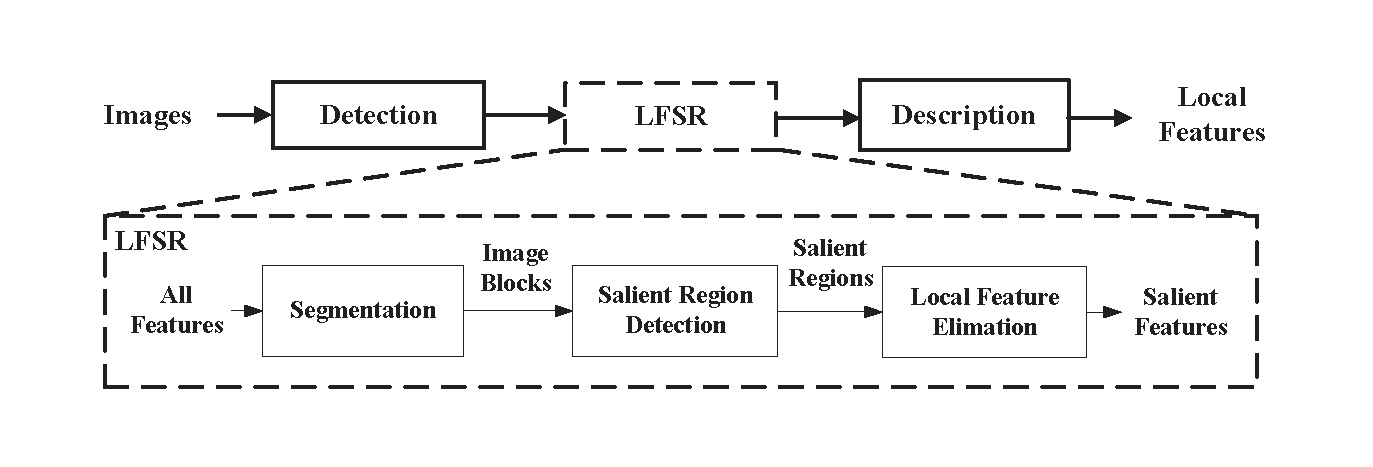
\includegraphics[width=4.5in]{images/fig-overview.eps}
\caption{An overview of {\sys}}
\label{fig:overview}
\end{figure*}

The basic motivation of {\sys} is to design a salient region detection algorithm, which can be used to optimize the obstacles of {\lfea}s and is easy to combined with them. Based on the observations in Section~\ref{subsec:observation}, we design and implement a local feature based salient region algorithm~({\sys}), which is efficient and easy to be combined with {\lfea}s.    

As shown in Figure \ref{fig:overview}, {\sys} works as a filter just between detection stage and description stage of a typical {\lfea}, where the input of {\sys} is detected feature points and its output is the sets of concerned feature points for computing feature vectors. There exist two major stages in our algorithm.
\begin{inparaenum}[\itshape a\upshape)]
\item First, a segmentation step is performed on all local features to identify and partition multiple salient region in an image. 
\item Second, for each image segmentation, {\sys} computes that segmentation's salient region individually based on the distribution information of the local feature points in it.
\end{inparaenum}


\subsection{Local Feature Based Segmentation}
\label{sec:algorithm_segmentation}

According to Observation~\ref{itm:observation_2}, an image may include several salient regions, which form multiple clusters of local features. We solve this problem by using a simple segmentation algorithm to divide the image into several blocks based on the distribution of local features. It scans along both the x axis and the y axis. In each scan, a cut-point may be found under the following two constraints:

\squishlist
\item \textit{No local feature could be divided into multiple parts.} In {\lfea}s, scale information is computed to guaranteed scale invariant. Therefore, a local feature point is used to represent a region with a radius that equals its scale as shown in Figure~\ref{fig:segmentation}. When the image is partitioned, no segmentation should across the region that a feature point representing.

\item \textit{The cut point should not locate far away form the center.} Each scan is performed from the region center. When the scan goes far, for example 1/4 of the region width, the scan stops and declares that there is no valid cut in that scan. This constraint attends to keep segmentation balanced and avoid too large or too small regions.
\squishend

A typical segmentation is shown in Figure~\ref{fig:segmentation}. The segmentation is started from the center of each axis, e.g. the dot lines in the figure. When a cut-point satisfying the above two constraints is found, The algorithm stops scanning and takes that cut-point as a valid image segmentation, e.g. the solid lines in the figure. After scanning on both the x axis and the y axis, at most four image regions are found in one segmentation.

\begin{figure}[!ht]
\centering
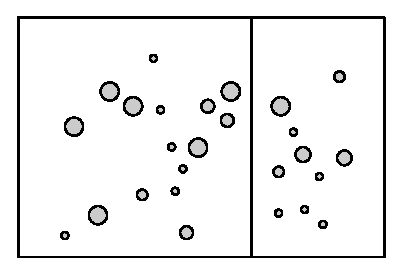
\includegraphics[width=2.1in]{images/fig-segmentation.eps}
\caption{Segmentation by scanning along both the x-axis and y-axis and starting from the dot lines and stops on the solid lines.}
\label{fig:segmentation}
\end{figure}

Then this kind of segmentation will be performed recursively on each image regions. And a recursive segmentation should stop when the following situations are satisfied:

\squishlist
\item \textit{No valid cuts are found.} When no valid cuts following the above two constraints are found, for example a scan exceeds its distance limit, on both x-axis and y-axis of a region, we should regard this region as a whole object and stop performing segmentation on it.

\item \textit{Too few features exist in a region.} Some found regions may have no local feature or just a few features, such as one or two local features, like gray regions in Figure~\ref{fig:segmentation-2}. These regions will be marked as invalid, because they cannot hold one whole object, and no further computation will be performed on them.

\item \textit{The number of segmentations exceeds the limitation.} It's possible that the recursive segmentation becomes too deep if there exist many dispersive points in that region. And actually it makes no sense to perform segmentation on these points, since they cannot be regarded as valid objects individually.

\squishend

\begin{figure}[!ht]
\centering
\includegraphics[width=2.1in]{images/fig-segmentation-2.eps}
\caption{Valid and invalid regions after two runs of segmentations. White regions are valid and gray regions are invalid.}
\label{fig:segmentation-2}
\end{figure}


According to our evaluation, in most cases two runs of segmentation are just enough, since almost no image has more than sixteen major objects. Thus, it's possible to simplify this processing by performing segmentation only twice in realistic scenarios.

\subsection{Salient Regaion Detection}
\label{sec:algorithm_detection}

As discussed in Section~\ref{sec:algorithm_overview}, a precise salient region detection is not suitable for local feature reduction in terms of processing speed and accuracy. Thus, {\sys} employs geometric meaning of local features to compute approximate salient regions.

According to Observation~\ref{itm:observation_1}, the local features in one salient region locate near to each other while noise or unimportant feature points locate far away from them. To simplify this problem, we regard the geometric center of feature points as the center of a salient region. Thus, the region center can be calculated based on the following equation:

{\begin{equation} \label{eq:center}
\left({x}_{c},{y}_{c} \right) = \frac{\sum_{i}^{N}\left({x}_{i},{y}_{i} \right)}{N}
\end{equation}}

Where $\left({x}_{c},{y}_{c} \right)$ means the geometric center of each local feature $\left({x}_{i},{y}_{i} \right)$ in that image segmentation.

After locating the center, we build the final salient regions by expanding the region as a rectangle with a particular width-length ratio. This ratio should be consistent with the distribution of local features, since local features always locate following the shape of target objects. Approximately, this ratio can be considered to equal to the ratio of the dispersion degree on x-axis and y-axis. For example, the bigger dispersion degree of local features on x-axis is, the bigger width-length ratio we will get. To compute the ratio of feature dispersions, we can divide the standard deviation of local feature position on x-axis by on y-axis:

{\begin{equation} \label{eq:ratio}
ratio = \sqrt{\frac{\sum_{i}^{N}\left ( x_{i}-x_{c} \right )^{2}}{\sum_{i}^{N}\left ( y_{i}-y_{c} \right )^{2}}}
\end{equation}}

Where $x_{i}$ and $y_{i}$ is a feature's position, while $x_{c}$ and $y_{c}$ is the center position computed by Equation~\ref{eq:center}. To get the final salient region, {\sys} grows the region size until the amount of local feature in it exceeds a desirable number, for example 50 percent of the original local features. As discussed in Observation \ref{itm:observation_3}, this threshold is important for providing a large enough salient region to avoid filtering local features on objects' edges and corners. In our evaluation, we find a ratio about 40\% is proper for most cases.

Combined with segmentation discussed in Section~\ref{sec:algorithm_segmentation}, the processing results will provide several candidate regions. According to Observation \ref{itm:observation_2}, we pick up the candidate regions that have at least 2 local features inside and regard them as the final salient regions.

\subsection{Local Feature Elimination}
\label{sec:algorithm_elimation}

With the knowledge of salient regions in an image, all features locate inside salient regions are kept for further computation, and all other features outside are just dropped. As a result, we get much fewer salient features in the local feature description stage, which can help to improve the whole algorithm's efficiency obviously.



\section{Related Work}

There exists many kinds of local feature descriptors. SIFT~\cite{lowe1999object}\cite{lowe2004distinctive} is the most publicly accepted and robust local feature-based image extraction algorithm. For different conditions or purposes, some variants of SIFT are also widely used, such as RIFT~\cite{lazebnik2005sparse}, GLOH~\cite{mikolajczyk2005performance}, and PCA-SIFT~\cite{ke2004pca}. To deal with the performance issue of SIFT, SURF~\cite{Bay2006SURF} is proposed in 2006 as a optimized local feature descriptor based on SIFT. With acceptable precision loss, SURF tends to be an efficient alternative of SIFT. Most of these algorithms are insensitive to various transformations, such as scaling, rotation and illumination.

Local feature descriptors are used widely because of their robust. Some researches focus on automatic image mosaic technique based on SIFT [9][11], stitching application of SIFT [10][15][12] and Traffic sign recognition based on SIFT [12].

Most salient region researches focus on generating precise salient map. Some of them~\cite{cheng2011global,achanta2009frequency} have already achieved impressive precision and recall. Since salient region is really helpful to local feature descriptors, researchers have also tried to combine them together. Huang et al.~\cite{huang2009image} involves a salient region detection algorithm by Itti et al.~\cite{itti1998model} to eliminate nosies for SURF descriptor. Liang et al.~\cite{liang2010salient} uses similar salient map method to perform noise reduction for SIFT descriptor. But none of them try to reuse local features for salient region detection or consider improve the computation performance of local feature descriptors.

\section{Evaluation}
\label{sec:evaluation}

In this section, we first present some comparisons on accuracy. Then, to show the performance improvement of local feature descriptor by using {\sys}, an evaluation is also performed on {\sys} combined with SIFT and SURF, two most widely used {\lfea}s.

\subsection{Experimental Comparison}
\label{sec:evaluation_comparison}

\begin{table}[!t]
\begin{center}
\begin{tabular}{|l|c|c|c|c|c|c|}
\hline
 & P & R & F1 & RE & SM(ms) & SG(ms) \\
\hline\hline
GBSR   & 0.81 & 0.86 & 0.83 & 39\% & 178 & 2086 \\
{\sys} & 0.52 & 0.59 & 0.55 & 42\% & N/A & 3.2 \\
\hline
\end{tabular}
\end{center}
\caption{Comparison between GBSR and {\sys} in precision (P), recall (R), F1 score, reduction efficiency (RE), saliency map (SM) and segmentation (SG) processing time in milliseconds.}
\label{tab:comparison}
\end{table}

As mentioned in Section~\ref{sec:introduction}, we target to design an algorithm for local feature reduction using salient region. To achieve good performance, an approximate salient region detection is involved. Although our approach cannot detect precise salient region, we are still interested in evaluating its precision against general purpose ones. Here we compare {\sys} with a previous research called GBSR (Global Contrast based Salient Region) by Cheng et al.~\cite{cheng2011global}. GBSR is a state-of-the-art salient region detection algorithm written in C++, which makes us easy to compare the computation efficiency with ours. To be used in feature elimination, we also perform GBSR's own segmentation approach to get the salient region boundary. It means in our evaluation the processing time of GBSR includes not only the saliency map detection but also the segmentation.

Since we only focus on local features, our evaluation differs from regular salient region researches: the precision and recall are given according to the results of local feature reduction, not the precise salient region boundary. The evaluated dataset is provided by Achanta et at.~\cite{achanta2009frequency}, which is a subset of the public image database from Liu et at.~\cite{liu2011learning}. As input, we first generate local features for the whole database with OpenSURF~\cite{evans2010opensurf}. 

As shown in the column 2, 3 and 4 of Table~\ref{tab:comparison}, {\sys} gets lower precision lower recall compared to GBSR. The reduction efficiency in the column 5 refers to the proportion of the left local features after a reduction. The results shows that both of them can help to eliminate more than half of the original features. As discussed in Section~\ref{sec:algorithm}, some limitations in our salient region detection approach prevents processing images with high texture background or overlapping objects correctly. With a obvious precision gap compared to the state-of-the-art approach, the salient region used in {\sys} is not suitable for general purpose scenarios.

To compare the efficiency of these two algorithms, we run {\sys} and GBSR both on a PC with one Intel Quad Core 2.4Ghz CPU and 4GB memory. The result in the column 6 of Table~\ref{tab:comparison} shows that the well optimized GBSR costs average 2086 milliseconds to get the final salient region for one image, while {\sys} only costs 3.2 milliseconds. Even only counting the time for saliency map detection, GBSR still needs average 178 milliseconds. The performance result of {\sys} is very impressive but not surprising, because the computation of {\sys} is really simple and straightforward.

\subsection{Local Feature Descriptor Integration}
\label{sec:evaluation_integration}

{\sys} is designed to improve the performance of local feature descriptor. To evaluate whether {\sys} satisfies this design purpose, we integrate our algorithm into the OpenSIFT~\footnote{http://robwhess.github.com/opensift/} and OpenSURF~\footnote{http://www.chrisevansdev.com/computer-vision-opensurf.html} to see the actual effects. The salient region detection is carefully added between the detection stage and the description stage. It means {\sys} can reuse the computation results directly from the detection stage. After the reduction of {\sys}, the computation of the description stage should be much smaller, since it's only related to the amount of local features.

Furthermore, we also implement a whole image retrieval system for evaluation. The system first builds a VOC-Tree~\cite{nister-stewenius-cvpr-2006} by using SIFT or SURF feature vectors extracted from image datasets. Then, each incoming query image is transfered into feature vectors too and compared in that VOC-Tree. At last, the found top similar images would be reordered by using RANSAC~\cite{ransac1981}. To involve {\sys}, we just replace the original local feature descriptor with a {\sys} enabled version.

The input for evaluation is an image retrial dataset by Nist\'er et al.~\cite{nister-stewenius-cvpr-2006} with 10200 VGA ($640\times480$ pixels) photos. And the whole experiment is performed on a server with a Intel Quad Core i7 3.4Ghz CPU and 4GB RAM. Table~\ref{tab:integration} shows the final performance results. Compared to the original local feature algorithm, {\sys} helps to improve the local feature descriptor performance by about 1.6X. And by reducing local features, the whole image retrieval system gains a more than 2X speedup in both building and query phase.

We also present the accuracy influence of introducing {\sys} to our retrieval system in the column 5 of Table~\ref{tab:integration}. Here, the retrieval results of different algorithms are scored following the method of Nist\'er et al.~\cite{nister-stewenius-cvpr-2006}. Then we get the accuracy by dividing the score of {\sys} enabled algorithms by of original ones. {\sys} based algorithms show a small accuracy loss of about 7 percent. Considering the great speedup provided by {\sys}, we regard this result as acceptable.

\begin{table}
\begin{center}
\begin{tabular}{|c|c|c|c|c|}
\hline
 & DES & BLD & QRY & ACY \\
\hline\hline
SIFT & 0.54s & 0.33s & 1.65s & - \\
SIFT-{\sys} & 0.33s & 0.12s & 0.77s & 93\% \\
\hline\hline
SURF & 0.15s & 0.06s & 0.54s & - \\
SURF-{\sys} & 0.09s & 0.03s & 0.34s & 94\% \\
\hline
\end{tabular}
\end{center}
\caption{Comparison between original {\lfea}s and {\sys} enabled ones. DES refers to {\lfea} time. BLD refers to VOC-Tree building time. QRY includes VOC-Tree query time and RANSAC time. ACY refers to the accuracy of the {\sys} enabled retrieval system compared to the original ones.}
\label{tab:integration}
\end{table}

\section{Conclusion}
\label{sec:conclusion}

In this paper, we present a Salient Region conducted Local Feature algorithm. With computing directly on local image features, {\sys} takes advantage of an approximate salient regions approach to perform local feature reduction. According to our evaluation, {\sys} can help to improve the performance of SURF descriptor with a 1.6X speedup. Furthermore, when used in a realistic image retrieval system, our algorithm improve the query performance more than 2 times. 

%\section*{Acknowledgement}

\label{sec:acknowledgment}

We thank the anonymous reviewers for their insightful comments. This work was funded by China National Natural Science Foundation under grant numbered 60903015, National 863 Program of China under Grant No. 2012AA010905, Key Project of National 863 Program of China under Grant No. 2009AA012201, Key Project of Major Program of Shanghai Committee of Science and Technology under Grant No. 08dz501600,  Fundamental Research Funds for the Central Universities in China and Shanghai Leading Academic Discipline Project (Project Number: B114).

%% REFERENCES
{\small
\bibliographystyle{ieee}
\bibliography{srlf}
}

\end{document}


